\section{期望与极限}
\label{sec:rvconv-expectation-limits}

$Y_n=n\,\mathbf{1}_{\{U<1/n\}}$几乎必然收敛到$0$，期望却恒为$1$：
\[
 \lim_{n\to\infty}\mathbb{E}[Y_n]=1\neq0=\mathbb{E}\Bigl[\lim_{n\to\infty}Y_n\Bigr] .
\]
随机变量趋近目标，少量的大取值仍然可以左右期望。期望与极限什么时候可以交换？本节依次研究三类条件给出的保证：单调的符号结构、一个共同的可积上界，以及对整族变量尾部的统一控制。

积分的单调收敛定理、Fatou引理与支配收敛定理已经在一般测度空间上证明，可参考\BookChapterRef{chap:integration}{卷四第6章“积分”}。期望就是概率测度下的积分，这些定理可以直接使用。本节的重点是解释每个条件在随机误差中起什么作用，以及去掉它时期望会怎样出错。

\subsection{单调收敛}
\label{sec:rvconv-monotone}

最容易的情形是变量单调增加。非负的量只增不减，取极限时不会丢掉已经累积的部分。

\begin{theorem}[单调收敛定理]
\label{thm:rvconv-monotone}
设随机变量$0\leq X_1\leq X_2\leq\cdots$几乎必然成立，且$X_n\xrightarrow{\mathrm{a.s.}}X$。则
\begin{equation}
 \lim_{n\to\infty}\mathbb{E}[X_n]=\mathbb{E}[X] ,
 \label{eq:rvconv-monotone}
\end{equation}
两边可以同时为$+\infty$。
\end{theorem}

这是卷四单调收敛定理在概率空间上的写法：在一个零概率事件之外，$X_n$逐点递增到$X$，把这个事件上的值改为零不改变任何期望。结论不要求$X$可积，极限期望允许是$+\infty$。

\paragraph{计数与Borel–Cantelli引理}
单调收敛最常见的来源是非负项的累计。设$A_1,A_2,\dots$是事件，前$n$个事件中发生的个数与总发生次数分别是
\[
 N_n=\sum_{k=1}^{n}\mathbf{1}_{A_k},\qquad N=\sum_{k=1}^{\infty}\mathbf{1}_{A_k} .
\]
$N_n$在每条记录上递增到$N$，$N$可以取$+\infty$。由期望的线性性，$\mathbb{E}[N_n]=\sum_{k\leq n}\mathbb{P}(A_k)$；再由定理~\ref{thm:rvconv-monotone}，
\begin{equation}
 \mathbb{E}\Bigl[\sum_{k=1}^{\infty}\mathbf{1}_{A_k}\Bigr]=\sum_{k=1}^{\infty}\mathbb{P}(A_k) .
 \label{eq:rvconv-count-mean}
\end{equation}

这给出Borel–Cantelli引理的另一个证明。若$\sum_k\mathbb{P}(A_k)<\infty$，则$\mathbb{E}[N]<\infty$；期望有限的非负随机变量几乎必然有限（否则在正概率事件上取$+\infty$，期望也是$+\infty$），所以几乎每条记录上只有有限个事件发生。“概率可和”就是“平均发生次数有限”。

\paragraph{极限期望可以是无穷}
反方向不成立：平均次数无穷，次数本身仍可能处处有限。取$A_k=\{U<1/k\}$。对给定的$U(\omega)>0$，$U<1/k$当且仅当$k<1/U$，所以
\[
 N_n=\min\Bigl\{n,\ \Bigl\lceil\frac1U\Bigr\rceil-1\Bigr\},\qquad N=\Bigl\lceil\frac1U\Bigr\rceil-1 .
\]
$N$在$U>0$时有限，即几乎必然有限。它的期望却是
\[
 \mathbb{E}[N]=\lim_{n\to\infty}\mathbb{E}[N_n]=\lim_{n\to\infty}\sum_{k=1}^{n}\frac1k=+\infty .
\]

\begin{BookInlineFigure}
 \centering
 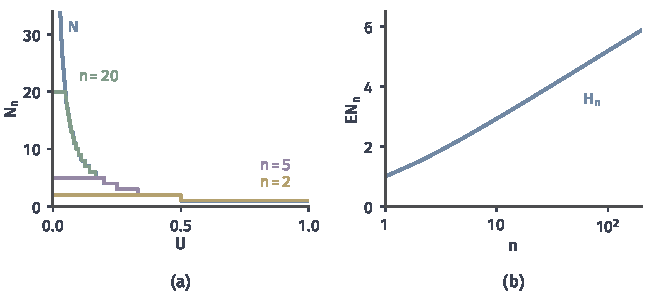
\includegraphics[width=112mm]{figures/07-probability/03-probability-limits/matplotlib/rvconv-monotone-count/figure.pdf}
 \caption{递增的计数变量$N_n=\sum_{k\leq n}\mathbf{1}_{\{U<1/k\}}$。(a)$N_n$作为$U$的函数，$n=2,5,20$（黄、紫、绿），蓝色台阶是极限$N=\lceil1/U\rceil-1$；各条台阶在$N\leq n$处与极限重合，只在$U$接近$0$处被截平。(b)$\mathbb{E}[N_n]=H_n=\sum_{k\leq n}1/k$，横轴为对数刻度。}
 \label{fig:rvconv-monotone-count}
\end{BookInlineFigure}

图~\ref{fig:rvconv-monotone-count}(a)中，$N_n$是极限$N$在高度$n$处的截平，截平的部分只在$U<1/n$这一小段上。随着$n$增大，截平的位置抬高，$N_n$下方的面积$H_n$一点一点地逼近$N$下方的面积。$N$在$U\to0$时像$1/U$那样增长，面积发散，(b)中$H_n\approx\ln n+0.577$随之无界增长。单调收敛定理正确地给出$\mathbb{E}[N]=+\infty$，它不需要极限可积。

\paragraph{单调性为何保留全部质量}
递增列不会丢掉期望的原因可以这样理解：每个$X_n$都在极限$X$的下方，且越来越贴近它。$X$的期望由它在各处的取值累积而成，任何一块有贡献的区域，迟早都会被$X_n$从下方填满，不存在“先出现、后消失”的贡献。

仅有非负性不够。$Y_n$非负且几乎必然趋于$0$，但不单调：$Y_n$在$\{U<1/n\}$上取$n$，在$Y_{n+1}$时这一块的大部分归零，又在更窄的$\{U<1/(n+1)\}$上取更大的值。图~\ref{fig:rvconv-spike-mass}在取值的数轴上画出它的分布：$Y_n$把质量$1/n$放在远处的$n$上，这一小块质量对均值的贡献恒为$n\cdot1/n=1$。随着$n$增大，这块质量越来越小、越来越远，极限中它消失了，它对均值的贡献却始终在。

\begin{BookInlineFigure}
 \centering
 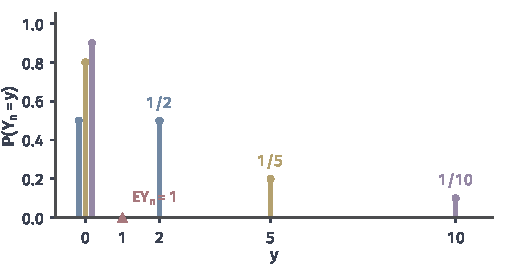
\includegraphics[width=86mm]{figures/07-probability/03-probability-limits/matplotlib/rvconv-spike-mass/figure.pdf}
 \caption{$Y_n=n\,\mathbf{1}_{\{U<1/n\}}$的分布，$n=2,5,10$（蓝、黄、紫）：质量$1-1/n$在$0$，质量$1/n$在$n$（$0$处的柱略微错开）。红三角是均值$\mathbb{E}[Y_n]=1$，对每个$n$都相同。}
 \label{fig:rvconv-spike-mass}
\end{BookInlineFigure}

\paragraph{递减的情形}
对递减列，单调性还需要配合可积性。若$X_n\geq0$递减到$X$且$\mathbb{E}[X_1]<\infty$，则$X_1-X_n$非负递增到$X_1-X$，对它用定理~\ref{thm:rvconv-monotone}，再从两边减去有限的$\mathbb{E}[X_1]$，得到$\mathbb{E}[X_n]\downarrow\mathbb{E}[X]$。

$\mathbb{E}[X_1]<\infty$不能省。取$X_n=U^{-1}\mathbf{1}_{\{U<1/n\}}$，它在$U>0$时递减到$0$，但对每个$n$，
\[
 \mathbb{E}[X_n]=\int_0^{1/n}\frac{\mathrm{d}u}{u}=+\infty .
\]
极限的期望是$0$，各项的期望都是$+\infty$。无穷减无穷没有意义，单调收敛定理只能用于递增的方向。

\subsection{Fatou引理}
\label{sec:rvconv-fatou}

不单调的非负列中，期望可以在极限里丢失，$Y_n$就是例子。但丢失只有一个方向：非负变量的质量可以逃到远处而消失，不能凭空产生。Fatou引理把这个单向的控制写成不等式。

\begin{theorem}[Fatou引理]
\label{thm:rvconv-fatou}
设随机变量$X_n\geq0$几乎必然成立，则
\begin{equation}
 \mathbb{E}\Bigl[\liminf_{n\to\infty}X_n\Bigr]\leq\liminf_{n\to\infty}\mathbb{E}[X_n] .
 \label{eq:rvconv-fatou}
\end{equation}
\end{theorem}

\begin{proof}
令$G_n=\inf_{k\geq n}X_k$。它非负，随$n$递增，极限是$\liminf_nX_n$。由定理~\ref{thm:rvconv-monotone}，
\[
 \mathbb{E}[G_n]\to\mathbb{E}\Bigl[\liminf_{n\to\infty}X_n\Bigr] .
\]

另一方面，对每个$k\geq n$都有$G_n\leq X_k$，所以$\mathbb{E}[G_n]\leq\mathbb{E}[X_k]$，对$k\geq n$取下确界，得到
\[
 \mathbb{E}[G_n]\leq\inf_{k\geq n}\mathbb{E}[X_k] .
\]
令$n\to\infty$，左边趋于式~\eqref{eq:rvconv-fatou}的左边，右边趋于它的右边。
\end{proof}

证明把一般的列换成它的尾部下确界，后者是递增的，于是可以用单调收敛。下确界只会比每一项都小，这就是不等式只有一个方向的来源。

\paragraph{严格不等号}
对$Y_n$，每条$U>0$的记录上$Y_n\to0$，所以式~\eqref{eq:rvconv-fatou}的两边是
\[
 \mathbb{E}\Bigl[\liminf_{n\to\infty}Y_n\Bigr]=0,\qquad \liminf_{n\to\infty}\mathbb{E}[Y_n]=1 .
\]
不等号严格成立，差额$1$正是逃到远处的那一块质量的贡献。概率越来越小、幅值越来越大的变量，总可以这样让极限的期望小于期望的极限。

\paragraph{非负性的作用}
把$Y_n$换成$-Y_n$，变量非正，几乎必然趋于$0$，而$\mathbb{E}[-Y_n]=-1$。这时
\[
 \mathbb{E}\Bigl[\liminf_{n\to\infty}(-Y_n)\Bigr]=0>-1=\liminf_{n\to\infty}\mathbb{E}[-Y_n] ,
\]
不等式反向。负的大值逃到远处时，带走的是负的贡献，极限的期望反而变大。所以Fatou引理需要下方的控制：非负，或者更一般地$X_n\geq-G$且$\mathbb{E}[G]<\infty$（对$X_n+G$用引理）。

\paragraph{极限的可积性}
Fatou引理最常用的形式是给极限的期望一个上界。若$X_n\xrightarrow{\mathrm{a.s.}}X$且$\sup_n\mathbb{E}[\lvert X_n\rvert]\leq C$，对$\lvert X_n\rvert$用式~\eqref{eq:rvconv-fatou}，得到
\begin{equation}
 \mathbb{E}[\lvert X\rvert]\leq\liminf_{n\to\infty}\mathbb{E}[\lvert X_n\rvert]\leq C .
 \label{eq:rvconv-fatou-bound}
\end{equation}
各项的平均绝对值一致有界时，极限必然可积。它只给出不等式，并不说明$\mathbb{E}[X_n]$收敛到$\mathbb{E}[X]$：$Y_n$满足$C=1$，极限的期望$0$严格小于$1$。

\subsection{支配收敛}
\label{sec:rvconv-dominated}

要得到等式，需要阻止质量逃逸。最直接的办法是给整列找一个共同的上界，并要求这个上界本身可积：所有变量都被关在同一个“有限面积”的笼子里。

\begin{theorem}[支配收敛定理]
\label{thm:rvconv-dominated}
设$X_n\xrightarrow{\mathrm{a.s.}}X$，并存在随机变量$G$，使$\mathbb{E}[G]<\infty$且对每个$n$都有$\lvert X_n\rvert\leq G$几乎必然成立。则$X$可积，且
\begin{equation}
 \lim_{n\to\infty}\mathbb{E}\bigl[\lvert X_n-X\rvert\bigr]=0,\qquad \lim_{n\to\infty}\mathbb{E}[X_n]=\mathbb{E}[X] .
 \label{eq:rvconv-dominated}
\end{equation}
\end{theorem}

\begin{proof}
取极限得$\lvert X\rvert\leq G$几乎必然，所以$X$可积，并且$\lvert X_n-X\rvert\leq2G$。于是$2G-\lvert X_n-X\rvert$非负，几乎必然趋于$2G$。由Fatou引理，
\[
 \mathbb{E}[2G]\leq\liminf_{n\to\infty}\mathbb{E}\bigl[2G-\lvert X_n-X\rvert\bigr]=\mathbb{E}[2G]-\limsup_{n\to\infty}\mathbb{E}\bigl[\lvert X_n-X\rvert\bigr] .
\]

$\mathbb{E}[2G]$有限，可以从两边消去，得到$\limsup_n\mathbb{E}[\lvert X_n-X\rvert]\leq0$，即平均绝对误差趋于零。最后，
\[
 \bigl\lvert\mathbb{E}[X_n]-\mathbb{E}[X]\bigr\rvert\leq\mathbb{E}\bigl[\lvert X_n-X\rvert\bigr]\to0 .
\]
\end{proof}

证明的关键是把误差$\lvert X_n-X\rvert$翻成$2G$减去它，后者非负，Fatou引理就从“只能变小”的单向控制变成了对误差的控制。可积性$\mathbb{E}[G]<\infty$用在消去$\mathbb{E}[2G]$这一步。

\paragraph{有界收敛}
概率空间的总质量为一，常数是可积的。所以若$\lvert X_n\rvert\leq c$对某个常数$c$成立，支配条件自动满足，这称为\term{有界收敛定理}（bounded convergence theorem）。累计最大值满足$0\leq M_n\leq1$，于是
\[
 \mathbb{E}[M_n]=\frac{n}{n+1}\to1=\mathbb{E}[1] .
\]
在一般测度空间上，常数在总测度无限时不可积，有界收敛不能这样直接得到。

\paragraph{依概率收敛下的支配收敛}
定理中的几乎必然收敛可以减弱为依概率收敛。设$X_n\xrightarrow{\mathbb{P}}X$，$\lvert X_n\rvert\leq G$，$\mathbb{E}[G]<\infty$，记$a_n=\mathbb{E}[\lvert X_n-X\rvert]$。由定理~\ref{thm:rvconv-subsequence}，有子列几乎必然收敛到$X$，取极限得$\lvert X\rvert\leq G$，$X$可积。

再看数列$(a_n)$的任意子列。由定理~\ref{thm:rvconv-subsequence-criterion}，它有进一步的子列使$X_n$几乎必然收敛到$X$，对这个子列用定理~\ref{thm:rvconv-dominated}，相应的$a_n$趋于零。一个实数列的每个子列都有趋于零的进一步子列，整个数列就趋于零，所以$a_n\to0$。

\paragraph{共同上界与包络}
$Y_n$为什么不满足定理？任何共同上界$G$都不小于包络$\sup_nY_n$。对$U(\omega)>0$，$Y_n(\omega)=n$当且仅当$n<1/U(\omega)$，所以包络就是第~\ref{sec:rvconv-monotone}小节的计数变量：
\[
 \sup_nY_n=\Bigl\lceil\frac1U\Bigr\rceil-1=N,\qquad \mathbb{E}[N]=+\infty .
\]
包络不可积，任何共同上界也不可积，支配收敛定理不适用，结论也确实不成立。

$Z_n=\sqrt n\,\mathbf{1}_{\{U<1/n\}}$的包络是$\sqrt N$。$N=n$当且仅当$1/(n+1)\leq U<1/n$，概率为$1/(n(n+1))$，所以
\[
 \mathbb{E}\bigl[\sqrt N\bigr]=\sum_{n=1}^{\infty}\frac{\sqrt n}{n(n+1)}=\sum_{n=1}^{\infty}\frac{1}{\sqrt n\,(n+1)}\approx1.860 .
\]
包络可积，支配收敛定理给出$\mathbb{E}[Z_n]\to0$，与直接计算的$n^{-1/2}$一致。

\begin{BookInlineFigure}
 \centering
 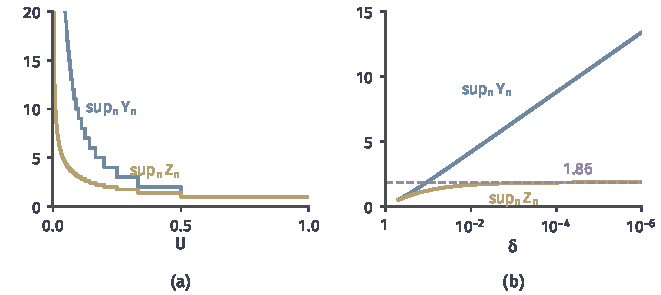
\includegraphics[width=112mm]{figures/07-probability/03-probability-limits/matplotlib/rvconv-envelope/figure.pdf}
 \caption{两族稀有大值的包络。(a)$\sup_nY_n=\lceil1/U\rceil-1$（蓝）与$\sup_nZ_n=\sqrt{\lceil1/U\rceil-1}$（黄）作为$U$的函数。(b)从$\delta$到$1$的积分随$\delta\to0$的变化，横轴为对数刻度且向右递减：蓝线按$\ln(1/\delta)$无界增长，黄线趋于$\mathbb{E}[\sqrt N]\approx1.86$（紫色虚线）。}
 \label{fig:rvconv-envelope}
\end{BookInlineFigure}

图~\ref{fig:rvconv-envelope}比较两个包络。两者在$U\to0$时都趋于无穷，差别在于增长的快慢：$\sup_nY_n$像$1/U$，下方面积发散；$\sup_nZ_n$像$U^{-1/2}$，下方面积有限。共同上界控制的不是单个变量，而是整族变量在稀有区域上能取到的最大值。

\paragraph{共同上界控制了什么}
共同可积上界的作用可以写成一个统一的尾部估计。若$\lvert X_n\rvert\leq G$，则$\{\lvert X_n\rvert>M\}\subseteq\{G>M\}$，在这个事件上$\lvert X_n\rvert\leq G$，所以
\begin{equation}
 \sup_n\mathbb{E}\bigl[\lvert X_n\rvert\,\mathbf{1}_{\{\lvert X_n\rvert>M\}}\bigr]\leq\mathbb{E}\bigl[G\,\mathbf{1}_{\{G>M\}}\bigr] .
 \label{eq:rvconv-envelope-tail}
\end{equation}
右边是单个可积变量的尾部贡献，$M\to\infty$时由支配收敛趋于零。共同上界真正做到的，是让整族变量在大取值处的贡献一起变小。下一小节把这一点单独拿出来作为条件。

\subsection{一致可积性}
\label{sec:rvconv-uniform-integrability}

$Y_n$的问题是平均被越来越稀有的大值维持着。要排除这种情形，应当要求大取值区域上的贡献对整族变量一致地小，而不必要求有一个共同的上界。

\begin{definition}[一致可积]
\label{def:rvconv-ui}
设$\{X_i:i\in I\}$是一族可积随机变量。若
\begin{equation}
 \lim_{M\to\infty}\ \sup_{i\in I}\ \mathbb{E}\bigl[\lvert X_i\rvert\,\mathbf{1}_{\{\lvert X_i\rvert>M\}}\bigr]=0 ,
 \label{eq:rvconv-ui}
\end{equation}
称这族变量\term{一致可积}（uniformly integrable）。
\end{definition}

单个可积变量$X$总满足这个条件：$\lvert X\rvert\mathbf{1}_{\{\lvert X\rvert>M\}}$被$\lvert X\rvert$控制，且在$\lvert X\rvert<\infty$处随$M\to\infty$趋于零，由支配收敛定理，它的期望趋于零。有限个可积变量也一致可积，对每个变量分别取$M$再取最大的那个即可。一致可积性的内容在于无穷多个变量同时满足，即同一个$M$对整族有效。

\paragraph{贯穿例子}
$Y_n$不一致可积。对任意$M$，当$n>M$时$\{Y_n>M\}=\{U<1/n\}$，所以
\[
 \mathbb{E}\bigl[Y_n\mathbf{1}_{\{Y_n>M\}}\bigr]=n\cdot\frac1n=1,\qquad
 \sup_n\mathbb{E}\bigl[Y_n\mathbf{1}_{\{Y_n>M\}}\bigr]=1 .
\]
无论阈值抬多高，总有某个$Y_n$把全部平均放在阈值之上。

$Z_n$一致可积。只有$\sqrt n>M$时$\{Z_n>M\}$才非空，此时它的贡献是$\sqrt n\cdot1/n=1/\sqrt n<1/M$，所以
\[
 \sup_n\mathbb{E}\bigl[Z_n\mathbf{1}_{\{Z_n>M\}}\bigr]\leq\frac1M\to0 .
\]
累计最大值在$[0,1]$中取值，$M\geq1$时贡献为零。图~\ref{fig:rvconv-ui-tails}画出三族的上确界随$M$的变化。

\begin{BookInlineFigure}
 \centering
 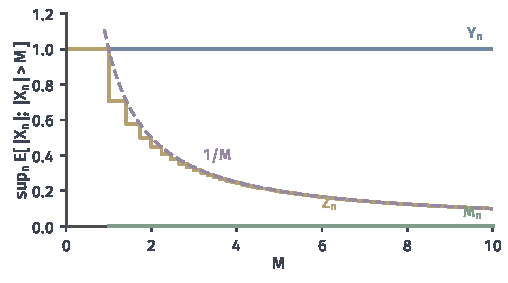
\includegraphics[width=86mm]{figures/07-probability/03-probability-limits/matplotlib/rvconv-ui-tails/figure.pdf}
 \caption{大取值区域上的一致贡献$\sup_n\mathbb{E}[\lvert X_n\rvert;\lvert X_n\rvert>M]$随阈值$M$的变化。蓝线：$Y_n$，恒为$1$，不一致可积。黄色台阶：$Z_n$，等于$1/\sqrt{\lfloor M^{2}\rfloor+1}$。紫色虚线：二阶矩给出的上界$\sup_n\mathbb{E}[Z_n^{2}]/M=1/M$。绿线：$M_n$，$M\geq1$时为零。}
 \label{fig:rvconv-ui-tails}
\end{BookInlineFigure}

\paragraph{判据}
直接验证式~\eqref{eq:rvconv-ui}往往不方便。下面三条比较常用的条件说明：共同可积上界和高于一阶的一致矩界都足够，而一阶矩一致有界本身不够。

\begin{theorem}[一致可积的充分条件]
\label{thm:rvconv-ui-criteria}
设$\{X_i:i\in I\}$是一族随机变量。
\begin{enumerate}
 \item 若存在$G$，$\mathbb{E}[G]<\infty$，使$\lvert X_i\rvert\leq G$对每个$i$几乎必然成立，则这族变量一致可积。
 \item 若存在$p>1$与$K<\infty$，使$\mathbb{E}[\lvert X_i\rvert^{p}]\leq K$对每个$i$成立，则这族变量一致可积，且
 \begin{equation}
  \sup_{i\in I}\mathbb{E}\bigl[\lvert X_i\rvert\,\mathbf{1}_{\{\lvert X_i\rvert>M\}}\bigr]\leq\frac{K}{M^{p-1}} .
  \label{eq:rvconv-ui-moment}
 \end{equation}
 \item 仅有$\sup_i\mathbb{E}[\lvert X_i\rvert]<\infty$不能推出一致可积。
\end{enumerate}
\end{theorem}

\begin{proof}
第1条即式~\eqref{eq:rvconv-envelope-tail}。

第2条。在$\{\lvert X_i\rvert>M\}$上，$\lvert X_i\rvert^{1-p}<M^{1-p}$，所以
\[
 \lvert X_i\rvert=\lvert X_i\rvert^{p}\cdot\lvert X_i\rvert^{1-p}\leq\frac{\lvert X_i\rvert^{p}}{M^{p-1}} .
\]
乘以$\mathbf{1}_{\{\lvert X_i\rvert>M\}}$再取期望，右边的期望不超过$\mathbb{E}[\lvert X_i\rvert^{p}]\leq K$，即得式~\eqref{eq:rvconv-ui-moment}。$p>1$保证右边随$M\to\infty$趋于零。

第3条。$Y_n$满足$\mathbb{E}[Y_n]=1$，但上面已算出它不一致可积。
\end{proof}

第2条中$p>1$是关键。$p$阶矩有界意味着大取值必须付出更高的代价：取值为$y$的部分在$p$阶矩中按$y^{p}$计入，在平均中只按$y$计入，所以平均的尾部被$p$阶矩以$M^{1-p}$的速度压住。$p=1$时这个比例是$1$，没有压缩，$Y_n$就钻了这个空子。$Z_n$满足$\mathbb{E}[Z_n^{2}]=1$，第2条给出上界$1/M$，正是图~\ref{fig:rvconv-ui-tails}中的紫色虚线。

同样的论证适用于任何增长快于线性的函数。若$\varphi\geq0$满足$\varphi(t)/t\to\infty$（$t\to\infty$），且$\sup_i\mathbb{E}[\varphi(\lvert X_i\rvert)]\leq K$，则在$\{\lvert X_i\rvert>M\}$上
\[
 \lvert X_i\rvert=\varphi(\lvert X_i\rvert)\cdot\frac{\lvert X_i\rvert}{\varphi(\lvert X_i\rvert)}\leq\varphi(\lvert X_i\rvert)\,\sup_{t>M}\frac{t}{\varphi(t)} ,
\]
于是尾部贡献不超过$K\sup_{t>M}t/\varphi(t)$，它随$M\to\infty$趋于零。例如$\varphi(t)=t\ln(1+t)$，它只比一阶矩多一个对数因子。反过来，每个一致可积族都存在这样的$\varphi$，这一方向的证明需要构造$\varphi$，篇幅较长，读者可查阅~\scite{math-kallenberg2021probability}。

\paragraph{小事件上的一致控制}
一致可积还有一个等价的说法：平均有界，并且在概率很小的事件上，整族变量的贡献一致地小。它把“大取值”换成了“小事件”，在证明中更方便。

\begin{lemma}[一致可积的等价刻画]
\label{lem:rvconv-ui-small-sets}
一族随机变量$\{X_i:i\in I\}$一致可积，当且仅当以下两条同时成立：
\begin{enumerate}
 \item $\sup_{i\in I}\mathbb{E}[\lvert X_i\rvert]<\infty$；
 \item 对每个$\eta>0$，存在$\delta>0$，使对每个满足$\mathbb{P}(A)<\delta$的事件$A$，
 \begin{equation}
  \sup_{i\in I}\mathbb{E}\bigl[\lvert X_i\rvert\,\mathbf{1}_{A}\bigr]<\eta .
  \label{eq:rvconv-ui-small-sets}
 \end{equation}
\end{enumerate}
\end{lemma}

\begin{proof}
必要性。把事件$A$按$\lvert X_i\rvert$是否超过$M$分成两块，第二块上$\lvert X_i\rvert\leq M$，所以
\[
 \mathbb{E}\bigl[\lvert X_i\rvert\,\mathbf{1}_{A}\bigr]\leq\mathbb{E}\bigl[\lvert X_i\rvert\,\mathbf{1}_{\{\lvert X_i\rvert>M\}}\bigr]+M\,\mathbb{P}(A) .
\]
给定$\eta>0$，先取$M$使第一项对所有$i$都小于$\eta/2$，再取$\delta=\eta/(2M)$，则$\mathbb{P}(A)<\delta$时左边小于$\eta$。取$A=\Omega$，第一项小于$\eta/2$，第二项是$M$，得到第1条。

充分性。记$C=\sup_i\mathbb{E}[\lvert X_i\rvert]$。由Markov不等式，
\[
 \mathbb{P}\bigl(\lvert X_i\rvert>M\bigr)\leq\frac{C}{M}\qquad\text{对每个 }i .
\]
给定$\eta$，取第2条中的$\delta$，再取$M>C/\delta$，则每个事件$\{\lvert X_i\rvert>M\}$的概率都小于$\delta$，由式~\eqref{eq:rvconv-ui-small-sets}，其上的贡献小于$\eta$，且对所有$i$同时成立。
\end{proof}

充分性中第1条不可缺：它保证事件$\{\lvert X_i\rvert>M\}$对整族一致地小，第2条才能用上。这个刻画说明，一致可积排除的正是“把平均藏在越来越小的事件里”。$Y_n$在概率$1/n$的事件上放下整份平均$1$，第2条对它不成立。

\subsection{\texorpdfstring{$L^{1}$}{L1}收敛的判据}
\label{sec:rvconv-l1-criterion}

现在可以回答本节开头的问题。依概率收敛缺的是尾部控制，一致可积恰好补上它，而且补得不多不少：在依概率收敛的前提下，$L^{1}$收敛与一致可积等价。

\begin{theorem}[Vitali收敛定理]
\label{thm:rvconv-vitali}
设$X_n\xrightarrow{\mathbb{P}}X$，且$\{X_n\}$一致可积。则$X$可积，且
\begin{equation}
 \lim_{n\to\infty}\mathbb{E}\bigl[\lvert X_n-X\rvert\bigr]=0,\qquad \lim_{n\to\infty}\mathbb{E}[X_n]=\mathbb{E}[X] .
 \label{eq:rvconv-vitali}
\end{equation}
\end{theorem}

这一结论称为\term{Vitali收敛定理}（Vitali convergence theorem）。卷四对有限测度空间的依测度收敛给出了一个按小区域估计的证明。这里换一种在概率论中更常用的写法：把每个变量截断成有界变量，有界部分用有界收敛，截掉的尾部用一致可积。对$M>0$，令
\[
 \varphi_M(x)=\max\{-M,\min\{x,M\}\} ,
\]
即把$x$限制在$[-M,M]$内。它满足两条性质：截断不会拉大两点的距离，截断误差只出现在阈值之外，
\[
 \lvert\varphi_M(x)-\varphi_M(y)\rvert\leq\lvert x-y\rvert,\qquad
 \lvert x-\varphi_M(x)\rvert\leq\lvert x\rvert\,\mathbf{1}_{\{\lvert x\rvert>M\}} .
\]
后一式左边等于$\max\{\lvert x\rvert-M,0\}$。

\begin{BookInlineFigure}
 \centering
 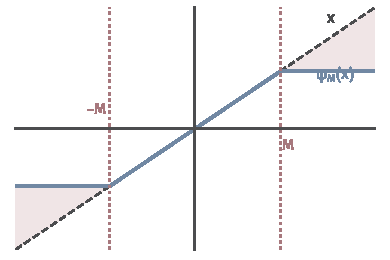
\includegraphics[width=66mm]{figures/07-probability/03-probability-limits/matplotlib/rvconv-truncation/figure.pdf}
 \caption{截断函数$\varphi_M$（蓝线，$M=2$）与恒等函数（灰色虚线）。两者只在$\lvert x\rvert>M$处不同，浅红区域的竖直高度就是截断误差$\lvert x-\varphi_M(x)\rvert=(\lvert x\rvert-M)^{+}$。}
 \label{fig:rvconv-truncation}
\end{BookInlineFigure}

图~\ref{fig:rvconv-truncation}画出截断误差的位置：它只出现在阈值之外，而一致可积说的正是阈值之外的贡献一致地小。

\begin{proof}
先证$X$可积。由引理~\ref{lem:rvconv-ui-small-sets}，$C=\sup_n\mathbb{E}[\lvert X_n\rvert]<\infty$。由定理~\ref{thm:rvconv-subsequence}，有子列$X_{n_k}\xrightarrow{\mathrm{a.s.}}X$，再由式~\eqref{eq:rvconv-fatou-bound}，$\mathbb{E}[\lvert X\rvert]\leq C$。

再估计误差。固定$M>0$，在$X_n$与$X$之间插入截断，由三角不等式，
\[
 \lvert X_n-X\rvert\leq\lvert X_n-\varphi_M(X_n)\rvert+\lvert\varphi_M(X_n)-\varphi_M(X)\rvert+\lvert\varphi_M(X)-X\rvert .
\]
取期望，逐项处理。

第一项是截掉的尾部，由截断误差的估计，
\[
 \mathbb{E}\bigl[\lvert X_n-\varphi_M(X_n)\rvert\bigr]\leq\tau(M),\qquad \tau(M)=\sup_k\mathbb{E}\bigl[\lvert X_k\rvert\,\mathbf{1}_{\{\lvert X_k\rvert>M\}}\bigr] .
\]
第三项同理不超过$\mathbb{E}[\lvert X\rvert\mathbf{1}_{\{\lvert X\rvert>M\}}]$。

第二项是有界部分。由$\varphi_M$的第一条性质，截断后的误差不超过原误差，所以$\varphi_M(X_n)\xrightarrow{\mathbb{P}}\varphi_M(X)$；同时它不超过$2M$。由依概率收敛下的有界收敛（第~\ref{sec:rvconv-dominated}小节），第二项的期望趋于零。于是
\[
 \limsup_{n\to\infty}\mathbb{E}\bigl[\lvert X_n-X\rvert\bigr]\leq\tau(M)+\mathbb{E}\bigl[\lvert X\rvert\,\mathbf{1}_{\{\lvert X\rvert>M\}}\bigr] .
\]

左边与$M$无关。令$M\to\infty$，第一项由一致可积趋于零，第二项因$X$可积而趋于零，所以平均绝对误差趋于零。期望的收敛与支配收敛定理的证明末尾相同。
\end{proof}

三个部分各有分工：依概率收敛只管有界的中间部分，一致可积管住所有$X_n$的尾部，$X$的可积性管住极限的尾部。缺了一致可积，第一项不能对所有$n$同时变小，$Y_n$就是这种情形：$\tau(M)=1$，误差停在$1$。

用贯穿例子核对。$Z_n\xrightarrow{\mathbb{P}}0$且一致可积，定理给出$\mathbb{E}[Z_n]\to0$，与直接计算的$n^{-1/2}$一致。移动区块与$\xi_n$都只取$0$和$1$，由第1条判据（$G=1$）一致可积，它们依概率收敛到$0$，所以也$L^{1}$收敛到$0$，与第~\ref{sec:rvconv-lp}小节的计算一致。

\paragraph{反方向}
$L^{1}$收敛的列一定一致可积，所以一致可积不只是充分条件。

\begin{theorem}[$L^{1}$收敛蕴含一致可积]
\label{thm:rvconv-l1-ui}
若$X_n\xrightarrow{L^{1}}X$，则$\{X_n\}$一致可积，且$X_n\xrightarrow{\mathbb{P}}X$。
\end{theorem}

\begin{proof}
依概率收敛是定理~\ref{thm:rvconv-implications}的第2条。一致可积用引理~\ref{lem:rvconv-ui-small-sets}验证。

平均有界。由三角不等式，
\[
 \mathbb{E}[\lvert X_n\rvert]\leq\mathbb{E}[\lvert X\rvert]+\mathbb{E}[\lvert X_n-X\rvert] ,
\]
右边第二项趋于零，所以左边有界。

小事件上的控制：对任意事件$A$，
\[
 \mathbb{E}\bigl[\lvert X_n\rvert\,\mathbf{1}_{A}\bigr]\leq\mathbb{E}\bigl[\lvert X\rvert\,\mathbf{1}_{A}\bigr]+\mathbb{E}\bigl[\lvert X_n-X\rvert\bigr] .
\]
给定$\eta>0$，取$N$使$n\geq N$时$\mathbb{E}[\lvert X_n-X\rvert]<\eta/2$。有限族$\{X,X_1,\dots,X_{N-1}\}$一致可积，由引理~\ref{lem:rvconv-ui-small-sets}，存在$\delta$，使$\mathbb{P}(A)<\delta$时其中每个变量在$A$上的贡献都小于$\eta/2$。

于是$\mathbb{P}(A)<\delta$时，$n<N$的项在$A$上的贡献小于$\eta/2$，$n\geq N$的项由上式小于$\eta/2+\eta/2=\eta$。
\end{proof}

两个定理合起来：在$X_n\xrightarrow{\mathbb{P}}X$的前提下，
\begin{equation}
 X_n\xrightarrow{L^{1}}X\quad\Longleftrightarrow\quad\{X_n\}\text{ 一致可积} .
 \label{eq:rvconv-l1-iff}
\end{equation}
依概率收敛与一致可积分别补上了第~\ref{sec:rvconv-comparison}节所说的两种缺陷中的一种：前者保证超差的机会消失，后者保证超差的大小不能维持平均。

\paragraph{\texorpdfstring{$L^{p}$}{Lp}收敛}
同样的判据适用于$p$阶矩。设$X_n\xrightarrow{\mathbb{P}}X$，$\{\lvert X_n\rvert^{p}\}$一致可积。由Fatou引理$X$的$p$阶矩有限，再由
\[
 \lvert X_n-X\rvert^{p}\leq2^{p-1}\bigl(\lvert X_n\rvert^{p}+\lvert X\rvert^{p}\bigr)
\]
和引理~\ref{lem:rvconv-ui-small-sets}，$\{\lvert X_n-X\rvert^{p}\}$也一致可积。它依概率收敛到$0$，由定理~\ref{thm:rvconv-vitali}，$\mathbb{E}[\lvert X_n-X\rvert^{p}]\to0$，即$X_n\xrightarrow{L^{p}}X$。

用$Z_n$核对$p=2$。$\{Z_n^{2}\}=\{n\,\mathbf{1}_{\{U<1/n\}}\}=\{Y_n\}$不一致可积，所以判据不能给出$L^{2}$收敛，而由式~\eqref{eq:rvconv-spike-moments}，$\mathbb{E}[Z_n^{2}]=1$，$Z_n$确实不$L^{2}$收敛。同一列变量$\{Z_n\}$一致可积而$\{Z_n^{2}\}$不一致可积，这正是第~\ref{sec:rvconv-comparison}节中$L^{1}$收敛与$L^{2}$收敛的分界。

\paragraph{期望收敛与平均误差}
最后要区分两件事：$\mathbb{E}[\lvert X_n-X\rvert]\to0$与$\mathbb{E}[X_n]\to\mathbb{E}[X]$。前者推出后者，后者推不出前者，因为期望是有符号的，正负误差可以互相抵消。取
\[
 W_n=n\,\mathbf{1}_{\{U<1/(2n)\}}-n\,\mathbf{1}_{\{1/(2n)\leq U<1/n\}} .
\]
它在$U>0$时最终为零，$W_n\xrightarrow{\mathrm{a.s.}}0$。正负两块各贡献$\pm1/2$，所以
\[
 \mathbb{E}[W_n]=\frac12-\frac12=0,\qquad \mathbb{E}\bigl[\lvert W_n\rvert\bigr]=\frac12+\frac12=1 .
\]

\begin{BookInlineFigure}
 \centering
 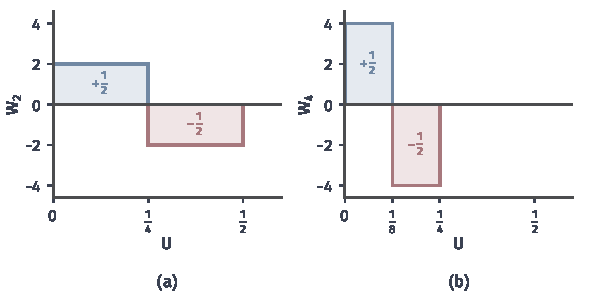
\includegraphics[width=100mm]{figures/07-probability/03-probability-limits/matplotlib/rvconv-signed-cancel/figure.pdf}
 \caption{正负抵消的变量$W_n$作为$U$的函数。浅蓝块是正的部分，面积$1/2$；浅红块是负的部分，面积$1/2$。(a)$n=2$。(b)$n=4$。期望恒为$0$，平均绝对误差恒为$1$。}
 \label{fig:rvconv-signed-cancel}
\end{BookInlineFigure}

图~\ref{fig:rvconv-signed-cancel}中正负两块面积相等，期望恰好是零，与极限$0$的期望相同；但两块的绝对面积加起来是$1$，平均绝对误差没有消失。$\{W_n\}$不一致可积，与$Y_n$同理。期望收敛只是一个数的收敛，平均绝对误差的消失才是误差本身在平均意义下的消失。

对非负变量，抵消不会发生，两者等价。

\begin{lemma}[Scheffé引理]
\label{lem:rvconv-scheffe}
设$X_n\geq0$，$X_n\xrightarrow{\mathbb{P}}X$，$\mathbb{E}[X]<\infty$，且$\mathbb{E}[X_n]\to\mathbb{E}[X]$。则$\mathbb{E}[\lvert X_n-X\rvert]\to0$。
\end{lemma}

\begin{proof}
依概率收敛的子列几乎必然收敛，所以$X\geq0$几乎必然。把绝对值拆成正部与负部，$\lvert a\rvert=a+2\max\{-a,0\}$，取$a=X_n-X$，得到
\[
 \mathbb{E}\bigl[\lvert X_n-X\rvert\bigr]=\bigl(\mathbb{E}[X_n]-\mathbb{E}[X]\bigr)+2\,\mathbb{E}\bigl[(X-X_n)^{+}\bigr] .
\]
第一项按假设趋于零。第二项中$0\leq(X-X_n)^{+}\leq X$，这里用到$X_n\geq0$；$(X-X_n)^{+}$依概率收敛到$0$，又被可积的$X$控制，由依概率收敛下的支配收敛，它的期望趋于零。
\end{proof}

这个结论称为\term{Scheffé引理}（Scheffé's lemma）。非负性让负部被极限$X$从上方压住，正部的大小又由期望之差决定，抵消无处藏身。$Y_n$也是非负的，但$\mathbb{E}[Y_n]=1$不趋于$\mathbb{E}[0]=0$，引理的条件不满足，这与它不$L^{1}$收敛一致。
